\section{General Least Squares (GLS)}
\subsection{Theory}
General Least Squares solves a linear, overconstrained system of equations by minimizing the squared residuals of each observation equation, with a weight matrix defining the variance AND covariance of each observation equation.  Note that the equations are the same as WLS, except the Weight Matrix ($W$) contains covariances.

*Note that if the scale of the variance-covariance in the weight matrix is known to be 1, then the computed reference variance should be inspected to ensure it passes the $\chi^2$ goodness of fit test.  If it passes the test, the Covariance matrix should NOT be multiplied by the reference variance.  See definition of reference variance for the reasoning.

\subsection{Assumptions}
\begin{itemize}
	\item No Outliers/Blunders WLS is not robust to outliers (consider RANSAC/Robust Weighting if outliers)
	\item System of equations is linear (eg. derivative wrt each unknown is not a function of any of the unknowns)
	\item System is over-constrained (eg. Number of Observation Equations > Number of Unknowns)
	\item Error only in dependent variable (eg. mx+b = y + v $\rightarrow$ error only in y dimension)
	\item Covariance between weight of each observation
\end{itemize}
\subsection{Equations}
\[
WAX=WL+WV 
\]
\[
m = \text{number of observations} \hspace{1cm} 
n = \text{number of unknowns}
\]
\[
dof = \text{degrees of freedom (\# of redundant observations)} = m-n
\]
\[
A = \begin{bmatrix}
a_{11} & a_{12} & \dots & a_{1n} \\
a_{21} & a_{22} & \dots & a_{1n} \\
\vdots & \vdots & \ddots& \vdots \\
a_{m1} & a_{m2} & \dots & a_{mn} \\
\end{bmatrix}
\hspace{0.5cm}
X = 
\begin{bmatrix}
x_1 \\ x_2 \\ \vdots \\ x_n
\end{bmatrix}
\hspace{0.5cm}
L = 
\begin{bmatrix}
l_1 \\ l_2 \\ \vdots \\ l_m
\end{bmatrix}
\hspace{0.5cm}
V = 
\begin{bmatrix}
v_1 \\ v_2 \\ \vdots \\ v_m
\end{bmatrix}
\hspace{0.5cm}
W = 
\begin{bmatrix}
\sigma_{11}^2 & \sigma_{12}^2 & \dots & \sigma_{1m}^2 \\ 
\sigma_{21}^2 & \sigma_{22}^2 & \dots & \sigma_{2m}^2 \\ 
\vdots & \vdots & \ddots& \vdots \\
\sigma_{m1}^2 & \sigma_{m2}^2 & \dots & \sigma_{mm}^2 \\ 
\end{bmatrix}
^{-1}
\]
\begin{align*}
	\text{Unknowns} &= \hat{X} = inv(A^TWA)A^TWL\\
	\text{Residuals} &= V = AX - L\\
	\text{Reference Variance} &= S_0^2 = \dfrac{V'WV}{dof} \\
	\text{Cofactor Matrix} &= Q_{xx} = inv(A^TWA) \\
	\text{Covariance Matrix of Unkowns} &= \Sigma_{xx} = S_0^2 \times Q_{xx} \\
	\text{Covariance Matrix of Observations} &= \Sigma_{\hat{l}\hat{l}} = A \Sigma_{xx} A^T \\
	\text{Standard Deviation of Solved Unknowns} &= \sigma_{\hat{X}} = \sqrt{diag(\Sigma_{xx})} \\
	\text{Predicted L} &= \hat{L} = AX \\
	\text{R$^2$ (model skill)} &= \dfrac{var(\hat{L})}{var(L)} \\
	\text{RMSE } &= \sqrt{\dfrac{VV^T}{m}} \\
\end{align*}
\clearpage

\subsection{Sample Problem}

Given the control coordinates $(x_c,y_c)$, corresponding measured coordinates $(x,y)$, and estimated covariance matrix of the control coordinates $\Sigma_c$: 
\[
x_c = [1,2,3] \hspace{1cm} y_c = [0, 5, 1]  \hspace{1cm} x = [6,1,8] \hspace{1cm} y = [3,12,8]
\]
\[
\Sigma_c = 
 \begin{bmatrix}
\sigma_{x_{c_1}x_{c_1}}^2 & \sigma_{x_{c_1}y_{c_1}} & \sigma_{x_{c_1}x_{c_2}} & \sigma_{x_{c_1}y_{c_2}} & \sigma_{x_{c_1}x_{c_3}} & \sigma_{x_{c_1}y_{c_3}}  \\ 
\sigma_{x_{c_1}y_{c_1}} & \sigma_{y_{c_1}}^2 & \sigma_{y_{c_1}x_{c_2}} & \sigma_{y_{c_1}y_{c_2}} & \sigma_{y_{c_1}x_{c_3}} & \sigma_{y_{c_1}y_{c_3}}  \\ 
\sigma_{x_{c_1}x_{c_2}} & \sigma_{y_{c_1}x_{c_2}} & \sigma_{x_{c_2}}^2 & \sigma_{x_{c_2}y_{c_2}} & \sigma_{x_{c_2}x_{c_3}} & \sigma_{x_{c_2}y_{c_3}}  \\ 
\sigma_{x_{c_1}y_{c_2}} & \sigma_{y_{c_1}y_{c_2}} & \sigma_{x_{c_2}y_{c_2}} & \sigma_{y_{c_2}}^2 & \sigma_{y_{c_2}x_{c_3}} & \sigma_{y_{c_2}y_{c_3}}  \\ 
\sigma_{x_{c_1}x_{c_3}} & \sigma_{y_{c_1}x_{c_3}} & \sigma_{x_{c_2}x_{c_3}} & \sigma_{y_{c_2}x_{c_3}} & \sigma_{x_{c_3}}^2 & \sigma_{x_{c_3}y_{c_3}}  \\ 
\sigma_{x_{c_1}y_{c_3}} & \sigma_{y_{c_1}y_{c_3}} & \sigma_{x_{c_2}y_{c_3}} & \sigma_{y_{c_2}y_{c_3}} & \sigma_{x_{c_3}y_{c_3}} & \sigma_{y_{c_3}}^2  \\ 
 \end{bmatrix}
 = 
 \begin{bmatrix}
 0.5 & 0.3 & 0 & 0 & 0 & 0 \\
 0.3 & 0.5 & 0 & 0 & 0 & 0 \\
 0 & 0 & 0.4 & 0.1 & 0 & 0 \\
 0 & 0 & 0.1 & 0.2 & 0 & 0 \\
 0 & 0 & 0 & 0 & 0.7 & 0.4 \\
 0 & 0 & 0 & 0 & 0.4 & 0.4 \\
 \end{bmatrix} 
\]

Calculate the 2D Conformal (Four Parameter Similarity Transform) to go from the measured coordinates to the control coordinates.  (Note that the block diagonal structure of this covariance matrix describes that the x and y coordinate are correlated to each other for each point, but there is no correlation between points).  The 2D Conformal equations are:

\begin{align*}
x_c &= (S\cos(\theta))x - (S\sin(\theta))y + T_x \\
y_c &= (S\sin(\theta))x + (S\cos(\theta))y + T_y \\
\end{align*}

By substituting: 

\begin{align*}
	a &= S\cos(\theta) \\
	b &= S\sin(\theta) \\
\end{align*}
Where:

\begin{align*}
	\theta &= \tan^{-1}(\dfrac{b}{a}) \\
	S &= \dfrac{a}{\cos(\theta)}
\end{align*}

The observation equations become:

\begin{align*}
	F: \hspace{1cm} x_c &= ax - by + T_x \\
	G: \hspace{1cm} y_c &= bx + ay + T_y \\
\end{align*}

Note that every $(x_a,y_a)\rightarrow(x,y)$ correspondence produces 2 observation equations.

\[
A = 
\begin{bmatrix}[1.5]
\ddx{F_1}{a} & \ddx{F_1}{b} & \ddx{F_1}{T_x} & \ddx{F_1}{T_y}\\
\ddx{G_1}{a} & \ddx{G_1}{b} & \ddx{G_1}{T_x} & \ddx{G_1}{T_y}\\
\ddx{F_2}{a} & \ddx{F_2}{b} & \ddx{F_2}{T_x} & \ddx{F_2}{T_y}\\
\ddx{G_2}{a} & \ddx{G_2}{b} & \ddx{G_2}{T_x} & \ddx{G_2}{T_y}\\
\ddx{F_3}{a} & \ddx{F_3}{b} & \ddx{F_3}{T_x} & \ddx{F_3}{T_y}\\
\ddx{G_3}{a} & \ddx{G_3}{b} & \ddx{G_3}{T_x} & \ddx{G_3}{T_y}\\
\end{bmatrix} =
\begin{bmatrix}
x_1 & -y_1 & 1 & 0\\
y_1 & x_1 & 0 & 1\\
x_2 & -y_2 & 1 & 0\\
y_2 & x_2 & 0 & 1\\
x_3 & -y_3 & 1 & 0\\
y_3 & x_3 & 0 & 1
\end{bmatrix} =
\begin{bmatrix}
6 & -3 & 1 & 0\\
3 & 6 & 0 & 1\\
1 & -12 & 1 & 0\\
12 & 1 & 0 & 1\\
8 & -8 & 1 & 0\\
8 & 8 & 0 & 1
\end{bmatrix}
\hspace{1cm}
X = 
\begin{bmatrix}
a \\ b \\ T_x \\ T_y 
\end{bmatrix}
\]
\[
L =
\begin{bmatrix}
F(X_1) \\ G(X_1) \\ F(X_2) \\ G(X_2) \\ F(X_3) \\ G(X_3) \\
\end{bmatrix} = 
\begin{bmatrix}
x_{a_1} \\ y_{a_1} \\ x_{a_2} \\ y_{a_2} \\ x_{a_3} \\ y_{a_3}
\end{bmatrix} = 
\begin{bmatrix}
1 \\ 0 \\2 \\5 \\3 \\1 
\end{bmatrix}
\hspace{1cm}
W = inv(\Sigma_c)
\]
Use the Equations and solve:
\begin{table}[H]
\centering
\begin{tabular}{|c|c|c|}
\toprule
$n = 4$& %NEWCOLUMN
$m = 6$& %NEWCOLUMN
$dof = 2$\\ %NEWROW
\midrule
$\hat{X} = $$
 \begin{bmatrix}
0.38\\
-0.35\\
-2.62\\
0.76\\
\end{bmatrix}
$
& %NEWCOLUMN
$V = $ $
 \begin{bmatrix}
-0.31\\
-0.21\\
-0.03\\
-0.07\\
0.20\\
-0.03\\
\end{bmatrix}
$
& %NEWCOLUMN
$S_0^2 = 0.16$ \\ %NEWROW
\midrule
$\Sigma_{xx} = $ $
 \begin{bmatrix}
0.00&-0.00&-0.00&-0.00\\
-0.00&0.00&0.01&-0.00\\
-0.00&0.01&0.08&0.01\\
-0.00&-0.00&0.01&0.07\\
\end{bmatrix}
$
& %NEWCOLUMN
$\sigma_{\hat{X}} = $ $
 \begin{bmatrix}
0.02\\
0.03\\
0.27\\
0.27\\
\end{bmatrix}
$
& %NEWCOLUMN
$\Sigma_{\hat{l}\hat{l}} = $ $
 \begin{bmatrix}
0.03&0.00&0.00&-0.01&0.01&0.01\\
0.00&0.04&0.01&-0.01&-0.01&0.02\\
0.00&0.01&0.06&0.01&0.02&-0.01\\
-0.01&-0.01&0.01&0.03&0.01&-0.00\\
0.01&-0.01&0.02&0.01&0.02&-0.01\\
0.01&0.02&-0.01&-0.00&-0.01&0.02\\
\end{bmatrix}
$
\\ %NEWROW
\midrule
$Q_{xx} = $ $
 \begin{bmatrix}
0.00&-0.00&-0.02&-0.03\\
-0.00&0.01&0.04&-0.02\\
-0.02&0.04&0.48&0.04\\
-0.03&-0.02&0.04&0.47\\
\end{bmatrix}
$
& %NEWCOLUMN
$\hat{L} = $$
 \begin{bmatrix}
0.69\\
-0.21\\
1.97\\
4.93\\
3.20\\
0.97\\
\end{bmatrix}
$
& %NEWCOLUMN
$R^2 = 1.1018$ \hspace{1cm} $RMSE = 0.18$\\ %NEWROW
\bottomrule
\end{tabular}
\end{table}

Interpret the results:
\begin{itemize}
	\item $\theta$ and $S$ values and their covariances can be calculated using equations: $\theta = \tan^{-1}(\dfrac{b}{a})$ and $S = \dfrac{a}{\cos(\theta)}$
	\item $R^2$ isn't really a valid metric here, the variance of the coordinate doesn't mean anything useful.
	\item Error is assumed to only be in the control coordinates
	\item We can use these results to transform other coordinates with uncertainty using GLOPOV
	\item The $S_0^2$ value is not near one, indicating the variance-covariance matrix may have over-estimated the predicted error of the control data. a $\chi^2$ goodness of fit test should be done to confirm this.  
\end{itemize}
\todo{legend is messed up}
\begin{figure}[H]
	\centering
	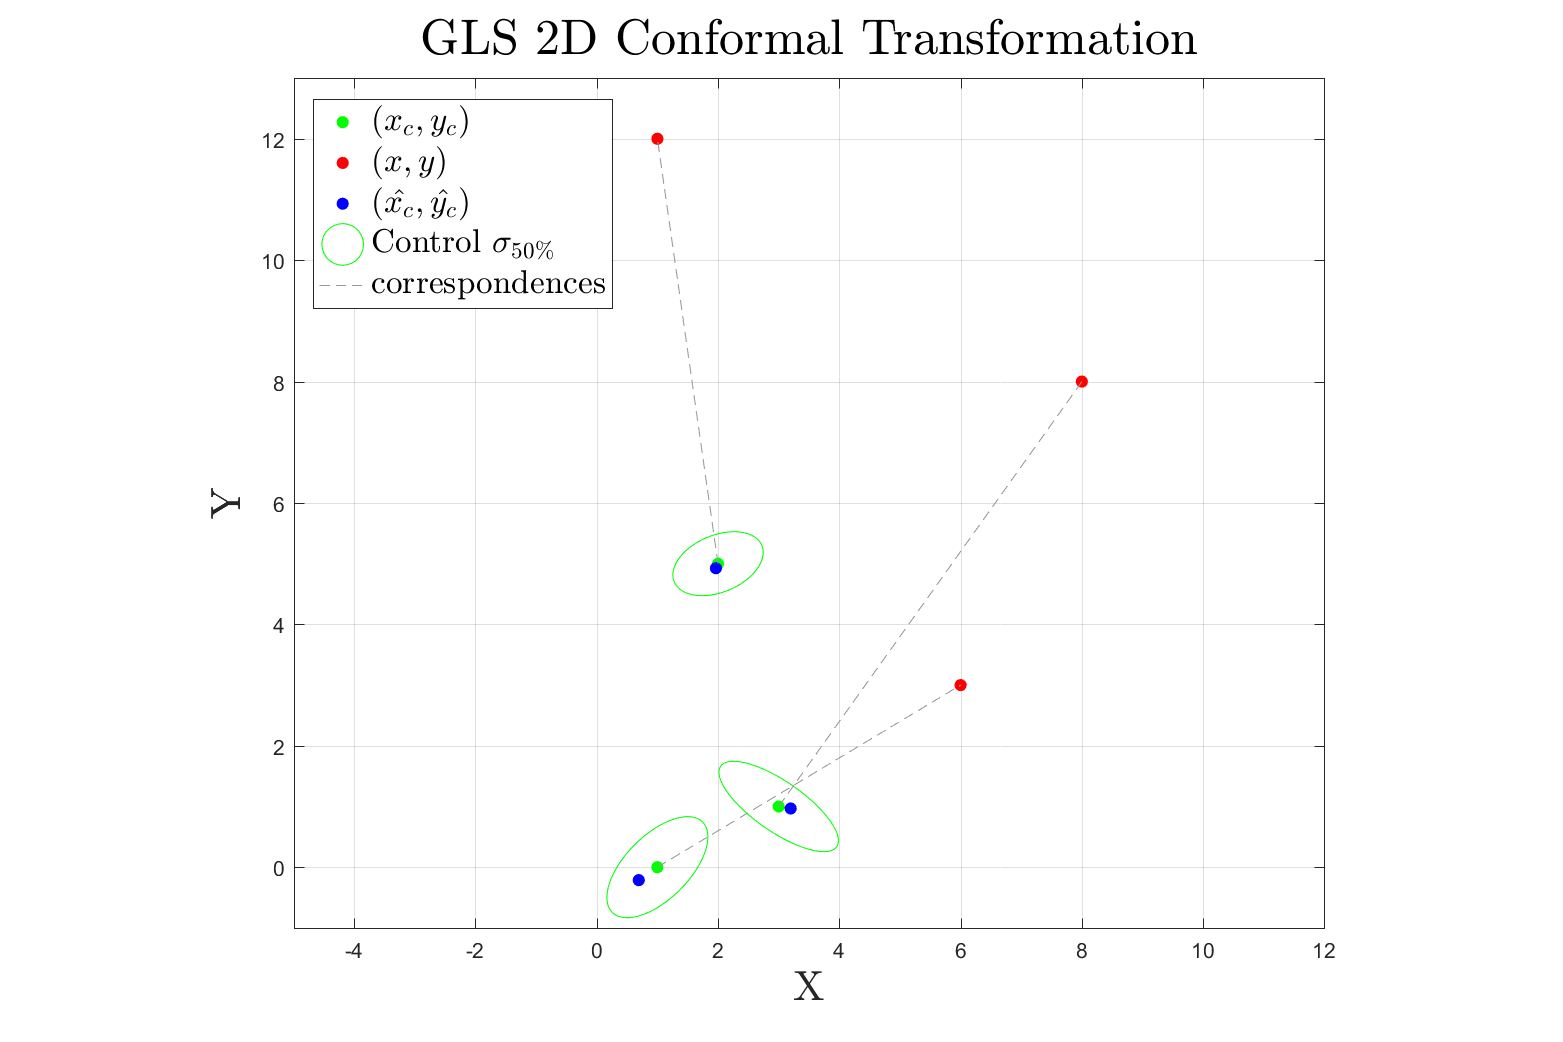
\includegraphics[height = 4in]{GLSexample.png}
\end{figure}
\clearpage
\subsection{Example Matlab Code}
\lstinputlisting[
label      = {alg:exampleGLS},
caption    = {exampleGLS.m},
style      = Matlab-editor,
basicstyle = \mlttfamily,
firstline  = 1,
lastline   = 39,
firstnumber= 1
]{exampleGLS.m}

\lstinputlisting[
label      = {alg:exampleGLS2},
caption    = {The Matlab built in function LSCOV generates the same results},
style      = Matlab-editor,
basicstyle = \mlttfamily,
firstline  = 41,
lastline   = 42,
firstnumber= 41
]{exampleGLS.m}



